\documentclass[a4paper,man,12pt,apacite]{apa6} % man => jou
\usepackage[english]{babel}
\usepackage[utf8]{inputenc}
\usepackage{mathtools}
\usepackage{url}
\usepackage{tikz}

\tikzset{
  treenode/.style = {align=center, inner sep=2pt, text centered,
    font=\sffamily, minimum size=0.5cm},
  arn_c/.style = {treenode, rectangle, draw=black},
  arn_d/.style = {treenode, ellipse, draw=black}
}

\begin{document}

\title{Random Forests Destructured: Introduction, Overview, Possibilities}
\shorttitle{Random Forests Destructured}
\author{Tobias Ammann}
\keywords{ensemble methods, introduction, random forests}
\affiliation{Literature Study at the Workgroup for Psychological Methods,\\Evaluation and Statistics, Department of Psychology.\\Supervised by Prof. Dr. Carolin Strobl}

\abstract{This report a rather new machine learning algorithm called
"Random Forests", its qualities, use, problems, and a small number of
improvements that have been tried.
Random forests are getting a lot of attention outside of psychology,
and it would be nice to encourage their application within psychology too.
However, it is important to keep in mind that random forests are
relatively unstudied. This hasn't hindered a number of people to suggest
improvements. This paper tries to give the reader a practical
understanding of the method, which hopefully leads to a better
application random forests.}

\keywords{ensemble methods, introduction, random forests}

\maketitle

\tableofcontents

\section{Introduction}

\subsection{Motivation}
Psychology has become a science, thus psychological research has to follow
the \emph{scientific method}, according to which positive proof is an
impossibility unless we have complete knowledge, and could eliminate all
alternative theories.
However, we won't ever have complete knowledge, therefore scientific isn't
about proofs, but probabilities.
Research works under the assumption that if we disprove just enough
alternative theories, we can eventually tell which theory is probably
true.
So, the scientific method really is nothing but the use of countless
attempts to disprove alternative theories, until only a single such theory
remains.

Since there is an unweildly number of theories to disprove, and every
researcher likes to see the result of his work during his lifetime, a
more speedy method is usually employed, although this comes with a caveat.
The speedier method has the researcher pit his favored theory against
the null hypothesis, a fancy word for chance.
This is way more efficient than comparing the thousands of
theories that researchers have come up with, and continue to come up with.
The caveat, commonly called confirmation bias, is that the result only
has significance in the experimental set-up being tested.
In the greater scale of things, i.e. reality, the results might well be
completely bogus.
Nonetheless, most of the subjects being studied are sufficiently constant
or change predictably enough to allow researchers to generalize from the
results of an experiment to the world at large, and likely remain correct.
This likelihood depends on the size of the effects measured in the
experiment, the number of experimental subjects, and on the properties of the
statistical methods involved.
In psychological research, where large effects are rare and
experiments usually study only a handful of psychology students, it is
vital to use good statistical methods, because that is the only parameter
remaining for the researcher to tweak in his favour.

Recently, researchers in psychology began to turn to a new breed of
statistical methods, in hope of ever better results. This new breed of
statistical methods is called \emph{machine learning}.

In this paper, I aim to introduce the reader to \emph{random forests},
which are just one family of algorithms.
I intend to do this in a way that gives every reader a chance to understand
this method without prior knowledge. I also intend to present the reader
with some context around random forests, in hope that they will benefit
from a more big-picture view.

In the next sections I introduce the reader to machine learning,
the differences between the traditional statistical and this new
machine learning approach, random forests in particular, and finally delve
into some improvements to random forests that have been suggested in the
literature.

\subsection{Machine Learning}
In order to understand random forests, it might be useful to set
the stage by briefly discussing machine learning in general.
Machine Learning is both a part of predictive statistics and the
artificial intelligence branch of computer science.

\emph{Predictive statistics} is the sub-field of statistics that is
concerned with making predictions based on past observations.
It's probably most widely known method is \emph{linear regression}
\cite{wpLR} that associates two variables \(y\) and \(x\) in such a way
that they describe a straight line: \(y = \alpha * x + \beta \).
Predictive statistics is widely used in psychology because it
allows the researcher to look at the unobservable by making
assumptions of the form \(reaction = mind * stimulus + variation\).
This is the standard approach in personality questionaires.

\emph{Artificial intelligence} is a field commonly associated with the
computer sciences, where it began with the advent of higher-order
programming languages based on mathematical foundations around the \emph{1960s} \cite{wpHOPL}.
Its aim is to give computers human-like capabilites, so that they can assist
us by combining intelligence, with flawless logic and super-human knowledge.
It includes things like \emph{logic programming} \cite{wpLP},
\emph{expert systems} \cite{wpES}, \emph{databases} \cite{wpDB} and
\emph{neural networks} \cite{wpNN}, that all represent some form of
storing and querying knowledge.
Unfortunately, early computers back then didn't have the speed and memory
required to push the envelope far enough, and the field was deemed dead.
Only the rather recent coexistance of powerful computers and massive amounts
of stored data, sometimes called \emph{big data}, revived artificial
intelligence as an important field of research.

\emph{Machine learning} is that part of artificial intelligence that
is concerned with the computer's learning of facts about the world.
These facts can then be stored and subsequently queried later on.
As such machine learning is concerned with making statements based
on past observations, and, is therefore, close to predictive statistics
\cite{wpML}.

\subsection{The Machine Learning Life Cycle}
This section discusses the difference between machine learning and traditional
statistical methods. Terminology.
The following section heavily relies on information found in Wikipedia, as
well as what I learned in statistics lectures in the past years.
A good introductory article is \cite{wpML}.

Traditionally, the statistical methods used in psychology
take a model of how the world works, and a set of data, and return one of
two things.
They either return a probability of how likely an improvement in prediction
can be observed at random, or how likely a difference in measurement can be
observed at random.

\emph{Regression methods} try to derive the values of
one variable from the other variables in the dataset using a formula the
researcher specifies.
They then compare the actual values and the prediction my the model with
different inputs, and calculate how probable an improvement in this
comparison is to show up due to random variations \cite{wpRA}.

\emph{Analysis of variance methods} partition the dataset
according to all but one variable. They then calculate the probability with
which the variation in the one variable among the groups could be due to
random variations in the dataset \cite{wpAOV}.

The probabilities the methods output are what statisticians call the
significance. Statisticians usually define a target significance level,
e.g. 5\%, and compare it to the output of their statistical calculations.
If the calculated probability is less than the targeted significance level the
measured effects are said to he significant at the chosen significance level.
For example, a result that is significant at 5\%, we know that it is less
likely to show up at random than in 5\% of all experiments.

The most striking difference between traditional statistical methods and
machine learning methods is that the researcher can't specify his model of
how the world works, other than through the selection of a machine learning
algorithm.
Because of this, machine learning algorithms are sometimes described as
\emph{black boxes}, meaning that the user can only see what's going into the
algorithm, and what is coming out.
This is unlike the statistical methods, where the researcher supplies a
formula, because in machine learning, algorithms derive the model on their own.
This is what the learning in machine learning means.
The second difference is what the algorithms return.
Since machine learning algorithms represent the model, what they output is
not a percentage, i.e. significance, but the model itself.
In short, machine learning provides the researcher with a generic model
that adapts to the world.
The prediction of such a model can then be calculated for data for which
the values of the output variable are known, but that hasn't
been included in the learning phase, to calculate the significance.
The problem with this flexibility is, that one cannot really tell what the
model looks like, that is, the model is not in a human-readable form.
As will be pointed out later, decision trees, the underlying mechanism in
random forests, are quite easily understandable, but random forests
consist of dozens to thousands of such trees, so that a human can hardly
tell what they mean.
Therefore, it is very important to find ways to condense this complexity
into something that can be more easily interpreted.
The variable importance measure of random forests, which will be introduced
later, is one such way.

\subsection{Classification}
The \emph{classification problem} is the problem of classifying new data based
on a set of example data, but without the explicit set of rules that guided the
classification of the example data.
Unlike in \emph{regression}, the result here is one of many given classes
and not a numeric value.
One might describe classification as regression with discreet output values.
Output variables are commonly called \emph{classes}, while input variables
are commonly called \emph{features} independent of the type of problem.

\subsection{Regression}
A short discussion of regression, the why and how, and the difference
between classical regression and regression in machine learning.
Terminology. Classification with continuous classes.

\subsection{Randomness}
Many machine learning algorithms consume random numbers in different places.
While computer generated random numbers are not truly random, they still
cause the outcome of the algorithm to change slightly between different
executions, due to the fact that they are customarily initialized with
the current time at the start of the program.
These changes might unnerve a novice, but don't change the outcome of the
algorithm significantly.
Still, for publication purposes it can make sense to set and publish the
random number generator's \emph{seed}, i.e. the value the generator is being
initialized with.
However, doing so during the experiment
is a serious mistake.
Indeed, it is good practice to run the analysis multiple times to ensure
that these random variations don't change the outcome.

% start of odt import

\section{Random Forests}

\subsection{Introduction}
This part of the paper discusses random forests.
“Random forests are a combination of tree predictors such that each tree
depends on the values of a random vector sampled independently and with
the same distribution for all trees in the forest” \cite{breiman2001random}.
Leo Breiman developed random forests with Adele Cutler, building on work
by Ho, Amit, Geman, and Dietterich \cite{wpRF}.

Although the name random forests is usually taken to refer to the random
forests as defined by \cite{breiman2001random}, the large number of
variants that have been derived from the original forests, e.g.
Forest-rk \cite{bernard2008forest}, RFW \cite{maudes2012random},
DRF \cite{bernard2012dynamic}, Fuzzy random forests \cite{bonissone2008fuzzy},
Rotation forest \cite{rodriguez2006rotation}, random forests that are
more random \cite{geurts2006extremely}, \cite{liu2005maximizing},
\cite{cutler2001pert}, and various other improvements, e.g. by
\cite{banfield2007comparison}, \cite{robnik2004improving},
\cite{strobl2009introduction}, \cite{zhang2012bias}, make it so that it
is better to think of random forests as being a framework instead of being
a single method \cite{wpRF}.
To understand this framework, it is best to look at the different aspects
of random forests, first in a top-down view, and later part by part.
The top-down view is strictly based on \cite{breiman2001random},
while the part by part discussion will also go into tweaking random forests.

Random forests is an ensemble learning method where the ensemble consists
of decision trees.
Every decision tree is constructed on a sample of the input dataset,
that is selected using bootstrapping with replacement from the original
dataset and equally large.
Every node split in the decision tree is an optimal two-way split selected
from a random subset of all input variables.
The number of randomly selected variables for each split is commonly called
\texttt{mtry}.
If the number of input variables is small, additional input variables can be
derived as linear combinations of input variables.
The decision trees are grown maximally without pruning,
and new trees are generated until the ensemble of decision trees reaches its
target size, usually called \texttt{ntree}.
Random forests features error estimates using out-of-bag data.
Out-of-bag data are the records in the dataset that were not selected during
the bootstrap aggregation, and make up approximately one third of the dataset.
Random forests also features variable importance measures,
which are calculated by reclassifying the out-of-bag data,
but randomizing the variable under consideration.
The variable importance of the randomized variable is the increase of
misclassifications.

The the reference implementation of random forests is written in Fortran,
but a package for the statistical software framework R \cite{rproject2012},
is called \texttt{randomForest} \cite{liaw2002classification} exists.
An alternative within the R framework, which includes improvements
to correct a bias in variable
importance measures is available under the name \texttt{party}
\cite{strobl2008conditional}.
A third implementation using Java is available in the WEKA machine learning
suite \cite{hall2009weka}.
For illustration purposes I include a source code example and the
corresponding output taken from \cite{strobl2008conditional}:

\begin{verbatim}
> load("dat_smoking.rda")
> library("party")
> myctree <- ctree(intention_to_smoke ~ ., data = dat_smoking)
> class(dat_smoking$intention_to_smoke)
> plot(myctree)
\end{verbatim}

The use case for random forests is quite wide.
Random forests has been used in applications from psychology and
computational biology as is outlined in \cite{strobl2009introduction},
to customer churn prediction \cite{xie2009customer},
to software testing \cite{guo2004robust} and internet security
\cite{zhang2005network}.
The reasons why random forests is such a widely used method,
are its prediction accuracy, which is comparable to other state-of-the-art
machine learning algorithms like Adaboost \cite{breiman2001random},
its ability to handle “small n large p” datasets \cite{strobl2009introduction},
its practical built in error estimates, and its variable importance measures.
The last of which, random forests' variable importance measures,
might be its most useful feature.
Many domains don't require accurate predictions as much as a model that can
be understood by humans.
While ensemble methods are unsuitably complex,
random forests' variable importance measures can be used to select variables
for use in simpler models, e.g.
generalized linear models, logit and probit models,
which are more easily interpreted \cite{strobl2009introduction}.

\subsection{Ensemble Learning Methods}
As mentioned above, random forests build on quite a rich collection of
previous work, most of which also concerns ensemble learning methods.
In fact, random forests can be seen as a composition of elements from
different other ensemble learning methods, e.g.
random subspaces \cite{ho1998random} and bagging \cite{breiman1996bagging}.
Although detailed knowledge of these methods is not a requirement to
understand random forests, it is important to understand what
ensemble learning is.
Again, this paper will first give an abstract definition and then look at
examples in detail.

Ensemble learning is a supervised learning algorithm: its task is to take
an example of input and output data, and find a hypothesis that connects
the two.
This hypothesis can then be used to predict the output data that
corresponds to new input data.
In theory this problem can be solved by a construct called
Bayes optimal classifier, which considers every possible hypothesis,
but, which unfortunately can't be implemented except for trivial problems.
However, the principle that the combination of possible hypotheses becomes
a stronger hypothesis, because it can represent more functions that every
component hypothesis could, holds.
In short, ensemble methods rely on the principle that the ensemble is more
than the sum of its parts.
The usual wording of this is, that ensemble learning turns a set of
\emph{weak classifiers} into one \emph{strong classifier}.
Weak also stands for unstable, meaning that the underlying classifier is
susceptible to even small variations in the input data.
Ensemble learning methods can be called meta algorithm,
because they rely on other simpler classifier algorithms,
and it is theoretically possible to create an ensemble learner for any
supervised learning algorithm. \cite{wpEL} \cite{Polikar:2009}

\subsubsection{Bagging}

The ensemble learning algorithm that most prominently underlies
random forests is bagging. Bagging stands for bootstrap aggregation.
Bootstrapping is a term that was used to describe
“[...] the process by which lumberjacks hoist themselves up trees [...]”
\cite{wpBOOT}.
In statistics it refers to the process of deriving additional samples
by resampling the original sample,
essentially simulating drawing additional samples from the population.
Bootstrap aggregation is an ensemble learning algorithm,
which trains each of its underlying weak classifiers on a different set
of input data created by bootstrapping.
It is another algorithm developed by Leo Breiman \cite{breiman1996bagging}.

Bagging is typically uses bootstrapping with replacement,
which leads the inclusion of on average two thirds of the original sample
in the derived sample.
Random forests uses the remaining third as out-of-bag data
\cite{breiman2001random}.

\subsubsection{Boosting}

Boosting is an ensemble method, where every weak classifiers gets to train
on the original sample, but the sample is improved with importance weights.
These weights are different for every weak classifier.
They are lower for records in the dataset that are correctly predicted by
the classifiers already in the ensemble,
and higher for records that classified wrongly.
In short, boosting focuses on eliminating one classification error after
another all data is classified correctly,
or a targeted ensemble size is reached.
This behavior makes boosting algorithms very fast learners,
but susceptible to errors in the dataset \cite{long2010random}.
Boosting isn't used in random forests as introduced by \cite{breiman2001random},
but there are variants who do, e.g.
dynamic random forests \cite{bernard2012dynamic}.
Adaboost \cite{freund1995decision} is probably the most popular
boosting algorithm, and the algorithm random forests in most commonly
compared to in terms of performance, e.g. \cite{breiman2001random},
\cite{banfield2007comparison} and \cite{rodriguez2006rotation}.

A large study \cite{banfield2007comparison} compared eight ensemble of
decision tree classifiers on 57 publicly available datasets and concluded
“[...] that boosting, random forests and randomized trees are
statistically significantly better than bagging.”

\subsection{Decision Trees}

The underlying algorithm of random forests is the decision tree classifier,
which is either a regression tree, or a classification tree.
The difference between the two types of trees is the type of output produced.
Classifications trees work with discreet output values,
while regression trees output a continuous numeric value.
For classification the most commonly chosen output value among an ensemble
of decision trees is assumed to be the right prediction.
For regression purposes the output of the ensemble is calculated by averaging
the outcomes the single trees.
As the name indicates, a decision tree is a tree data structure, i.e.
a set of nodes that are connected in a forward manner allowing branching,
but not cross links and circles.
Decision trees usually are binary trees, meaning that each node either has
two child nodes, or is a leaf node.
Each node represents a decision criterion, each edge a criterion match or
mismatch, and each leaf node an outcome of the represented decision tree.
Tree data structures are typically drawn from top to bottom.
For example, the following decision tree takes three numeric features
\texttt{a}, \texttt{b}, \texttt{c} to predict a discreet output variable
\texttt{class} with four possible values.

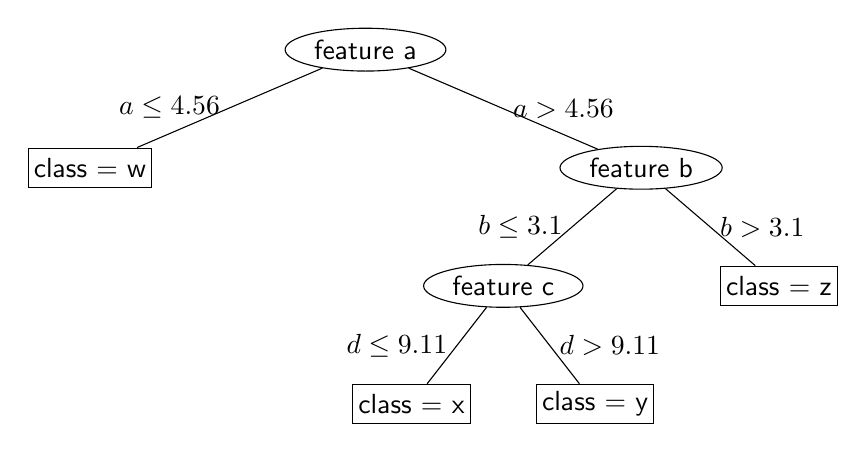
\begin{tikzpicture}[level/.style={sibling distance = 7cm/#1}]
\usetikzlibrary{shapes}
\usetikzlibrary{arrows}
\node [arn_d] {feature a}
    child{ node [arn_c] {class = w} edge from parent node[left] {\(a \le 4.56\)} }
    child{ node [arn_d] {feature b}
        child{ node [arn_d] {feature c}
            child{ node [arn_c] {class = x} edge from parent node[left] {\(d \le 9.11\)} }
            child{ node [arn_c] {class = y} edge from parent node[right] {\(d > 9.11\)} }
            edge from parent node[left] {\(b \le 3.1\)}
        }
        child{ node [arn_c] {class = z} edge from parent node[right] {\(b > 3.1\)} }
        edge from parent node[right] {\(a > 4.56\)}
    }

;
\end{tikzpicture}

The decision trees used by random forests are constructed by randomly
selecting a certain number of input variables as configured by the parameter
\texttt{mtry} for each node.
The algorithm then selects the best threshold among these input
variables as the node's criterion.
This process is repeated for every child node until a node is reached
which only matches records in the dataset with the same output value.
This node becomes a leaf node.
This is described as growing a tree maximally.
This ensures that each decision tree has a high strength,
meaning no decision tree outputs wrong predictions for the subsets of data
it matches. \cite{breiman2001random}

As a component classifier to an ensemble learning algorithm,
every decision tree should be different from the other decision trees in
the ensemble, i.e. the decision trees should be unstable,
to cover a wide range of possible interactions between the input data,
i.e. hypotheses.
This is commonly described as the trees being uncorrelated.
Tree strength and inter-tree correlation are what the prediction accuracy
of random forests depends on. \cite{breiman2001random}

The procedure by which decision trees are grown is modified by some
variants of random forests.
PERT \cite{cutler2001pert} for example doesn't perform a search for
the best split on a random selection of input variables,
but selects variable and threshold at random, while RFW \cite{maudes2012random}
searches all variables but attaches random weights to them,
and DRF \cite{bernard2012dynamic} influences the decision tree creation
by a procedure inspired by boosting.
Other variants, e.g. \cite{van2012accelerating}, change this procedure to
grow smaller or more balanced trees, to meet performance or
hardware requirements.

\subsection{Random Forests}
As has been described in the sections on ensemble learning and decision trees,
random forests build up ensembles of decision trees.
This process depends on two parameters: the ensemble size, commonly called
\texttt{ntree}, and the randomization parameter \texttt{mtry}.
Actually, random forests depend on another parameter,
the state of a random number generator, but being random,
it doesn't and usually shouldn't be specified.
The following is an exemplary implementation of random forest following the
original version by \cite{breiman2001random}.

\begin{verbatim}
TODO: Implementation of Random Forests
\end{verbatim}

\subsubsection{Parameters}
The two parameters random forests depends on, are problematic,
in that users set them according to one recommendation or another,
or just use the default setting, which again can differ from implementation
to implementation.
Furthermore, not every dataset is best learned by random forests using the
same setting.
This lack of a standard way to determine the parameter values makes it hard
to compare the accuracy of different methods.
The comparative study by \cite{banfield2007comparison} gives a nice overview
over the datasets used in previous publications,
among which are \cite{breiman2001random} and \cite{dietterich2000ensemble},
that each used ensemble sizes of 50-200, and applied the algorithms being
compared to 18-27 datasets.
In each case the authors concluded that their method was superior to the
other methods in the study.
However, the more recent study by \cite{banfield2007comparison} found
“no stat. sig. improvement over bagging in 38 of 57 data sets”
when ensemble sizes of up to 1000 trees where used.
The study also concludes that bagging with an ensemble size of 1000 and
random forests with the randomization parameter set to the
binary logarithm of the number of input variables were the best methods.
The study by \cite{banfield2007comparison} also suggests a mechanism
to determine the best size of the ensemble automatically.
Methodologically, this would be a welcome improvement, because it takes
away one way researchers can fiddle with the outcome of their calculations,
and because it would ensure better results due to the usually larger
ensemble sizes.
In defense of older studies, like those by \cite{breiman2001random} and
\cite{dietterich2000ensemble}, one has to consider that the average
computer back then weren't as powerful.
\cite{breiman2001random} mentions run times for random forests of 4 minutes
and 3 hours for Adaboost when building ensembles of size 100,
while I can execute all examples in \cite{strobl2009introduction}
in well under 30 seconds.

The second parameter of random forests is the randomization parameter
\texttt{mtry} which controls how many variables are being selected randomly
at each decision tree node to search for an optimal split.
If \texttt{mtry} is set to 1, random forests acts like a linear combination
of the input variables.
If \texttt{mtry} is set to the number of variables, random forest becomes
bagging as proposed by \cite{breiman1996bagging}.
Common choices for \texttt{mtry} are 1, 2, and other small values in
older studies, e.g. \cite{breiman2001random}, and the square root of n,
or the binary logarithm of n, with n being the number of input variables,
becoming increasingly popular in newer literature, e.g.
\cite{strobl2009introduction}.
As mentioned above, using the binary logarithm of the number of
input variables is indeed the best choice for most datasets
\cite{banfield2007comparison}.
However, depending on the dataset and the ensemble size, \texttt{mtry}
needs to be chosen differently.
For example in studies of genetics, where the dataset often includes many
irrelevant input variables in addition to the dataset being a
“small n large p case”, it is necessary to use a larger value
for \texttt{mtry}, else some variables might never be used in the ensemble
at all \cite{strobl2009introduction}.
It might be interesting to consider choosing \texttt{mtry} automatically,
and two obvious suggestions for that would be to choose a random \texttt{mtry}
value for every decision tree being grown, or to use a function of the
number of input variables satisfying some statistical distribution criterion.
According to \cite{bernard2008forest} a greedy search or choosing one of
the values discussed above is the usual approach in the literature.
The same paper shows, that this doesn't have to be the case, by demonstrating
a "push-button" method that automatically derives a suitable value for
\texttt{mtry} and "is at least as statistically significant as the original".

\subsubsection{Out-of-bag Data}
Because random forests is based on bagging and uses bootstrapped samples,
each tree has a set of approximately one third of the original dataset
that has not been used to grow the tree.
This set can be used to test the prediction accuracy of each tree,
and the prediction accuracy of all trees can then be averaged to give an
error estimation of the entire random forest.
This out-of-bag error estimation is more precise than the standard error
estimate, which is using all of the dataset \cite{strobl2009introduction}.
This said, one should not forget that out-of-bag data isn't the
same thing as a genuine test dataset.
Depending on the size of the dataset, and the ensemble size, the downsides
of bootstrapping might shine through, and lead to an underestimation of
the prediction accuracy.

\subsubsection{Variable Importance}
As has been mentioned above, random forests have a built in variable
importance measure, which is calculated, by permutating the input variable
in the out-of-bag data of every tree, and calculating a new error estimate.
The difference between the out-of-bag error estimates with and without
randomly permutated input variable is the variable importance.
The more important a variable is, the more drastically the prediction error
increases when the variable is being randomized.
The variable is sometimes scaled, i.e. z-standardized,
but because it strongly depends on the parameter of random forests,
it's not possible to compare these variable importances across studies,
hence there is little use in doing so \cite{strobl2009introduction}.

The idea behind this way of calculating variable importances is,
that one would like to compare a prediction model with and without a
particular input variable to measure the variable's impact.
Obviously, one can't ignore all trees that incorporate a variable,
because each tree incorporates multiple input variables, and their impact
on the prediction would be modified too.
By randomly permutating the values of an input variable,
the variable's characteristics don't change, but the connection to the
output variable is broken.
However, according to \cite{strobl2007bias} the variable importance might
still depend on which variable is being measured, because this
variable importance measure is biased towards variables with many categories
and variables with many missing values.
Numeric variable usually have as many different values as there are records
in the dataset, meaning that their importance measure is greatly biased due
to the large number of “categories”.
Fortunately, this can be fixed, but “Only when subsamples drawn without
replacement, instead of bootstrap samples, in combination with unbiased
split selection criteria, are used in constructing the forest, can the
resulting permutation importance be interpreted reliably”
\cite{strobl2007bias}, although correlated input variables still are
problematic.
The R package party includes two functions, \texttt{ctree} and
\texttt{cforest}, that are not affected by this bias, due to
yet another variable importance termed “conditional variable importance”
\cite{strobl2008conditional}.
Correlated variables can be problematic, because trees that include a
pair of correlated input variables are less affected by the random
permutation of one of them.
Conditional variable importance considers these correlations.
However, \cite{gromping2009variable} argues, that this can't be avoided
as long as \texttt{mtry} is smaller than the number of input variables,
and that considering all input variables, i.e. bagging,
“might already go a long way” towards remedying the problem,
although due to the “large p small n case”, “unbiased estimation of all
coefficients is impossible” in any case.

Another problem that the variable importance measure can be affected by,
is that some variables might not be well represented in a random forest.
This can be due to a small setting for \texttt{mtry} and or \texttt{ntree}
in the presence of many irrelevant input variables, as often is the case
in genetics datasets, or if variables show perfect higher order effects,
i.e. interaction effects, but no main effects.
The latter is called the XOR problem.
It is important to note, that random forests with a different split selection
algorithm don't have to be affected by this, e.g. PERT \cite{cutler2001pert}.

Last but no least, both \cite{strobl2009introduction} and
\cite{gromping2009variable} see one of the advantages of random forests in
their variable importance measure.
\cite{gromping2009variable} compares linear variable importance measures
with the one built into random forests, and finds that the latter are
heavily dependent on the mtry parameter.
The larger \texttt{mtry} is, the better the importance estimates become.
Variable importance measures are used to select input variables for a simpler
model, e.g. a generalized liner model, which is more interpretable than a
forest of decision trees \cite{strobl2009introduction}.
Variable importance measures are also the probably only simple way to
“shed some light into the black box of random forests”
\cite{gromping2009variable}.
A alternative, but rather naive way to estimate variable importance is to count
the occurance of a variable over all trees \cite{strobl2009introduction}.
Other imaginable ways to estimate variable importance would be to use
algorithms that analyze the structure of each decision tree.
Another interesting point to make, is that random perturbation of an input
variable could in theory be used as part of many other models, including but
not limited to generalized linear models.

The way variable selection based on the variable importance measure is
being done, is by finding variables whose randomization led to an improvement
in prediction accuracy.
These improvements are just random effects, and function as an indicator
for which variable importances are within the random fluctuations,
and which are true indicators for important variables.

\subsubsection{Regression}
Random forest can not only be used for classification, but also for regression.
To produce the numeric output values necessary in regression,
the vote on the most popular output class in the forest is replaced by an
average calculation over all tree outputs.
One problem with regression using random forests is that more decision trees
end up covering the middle of the range of values of an output variable.
This means, that the prediction accuracy is good in the middle of the range
of values, but the predictions for extremer values become more and more
inaccurate \cite{zhang2012bias}.
The same paper also suggests five ways to estimate and reduce this bias.

% end of odt import

\section{Method}

\subsection{Selection of Papers}
I started my research on \emph{random forests} by reading the
introductory paper suggested by my supervisor titled
\emph{An introduction to recursive partitioning: Rationale, application
and characteristics of classification and regression trees, bagging and
random forests} \cite{strobl2009introduction}.
I then searched the research databases \emph{PsychARTICLES} and
\emph{PsychINFO} querying for \emph{random forest} and limiting my results
to the last two years.
I only considered papers that focus on \emph{random forests} and
dismissed every paper where \emph{random forests} are merely used as a
research method.
I also used \emph{Google Scholar} to look for more technical
publications outside the field of psychology.
I searched for combinations of \emph{random forest}, \emph{comparison},
\emph{analysis}, and \emph{ensemble}.
I also included keywords seen in interesting titles, like \emph{fuzzy},
\emph{perfect}, \emph{full}, \emph{balanced}, \emph{extremely}, and
\emph{rotation}.
I also queried for some of the referenced publications while I read the
found material, but only included \cite{strobl2008conditional}, because
it was referenced multiple times, and co-authored by this paper's
supervisor.

The final criteria for inclusion were the online availability of a freely
downloadable PDF-file, which thanks to \emph{Google Scholar} often turned
out to be no problem at all, and my decision on the topic of
this report.

A lot of the information in the fields of computer science, artificial
intelligence, machine learning, databases, and especially programming
I acquired through different means in the last ten years.
As I couldn't remember the original sources, I can only include the pages
on Wikipedia, which I used to refresh my memories.

\subsection{Aim and Structure of the Paper}
Possible options for this topic were the presentation of
exemplary uses of random
forests, the discussion of strengths and weaknesses, and any of the more
specialized variants.
During my research I had the impression, that there were serious
differences in the understanding of random forests among researchers,
and even among designers of improved variants.
A study comparing different decision tree ensemble techniques also confirmed
this expression by saying that many of the commonly used methods of comparison
weren't robust enough for use with random forests \cite{banfield2007comparison}.

Because of this fuzziness, I decided on a different focus, and to write
a very broad - big picture - introduction to random forests.

\section{Conclusion}
State of the art? Well... They are not yet properly understood, and
many comparisons and lots of the advantages might be accidential.
Strong dependance on parameters, with no rationally pleasing way to set them.

\subsection{The End}
Bye.

\bibliography{references}

\end{document}

